% =====================================================================
%  (c) Agent-Centric Video Encoder -- target-conditioned 3D cross-attention
%  Compile:  pdflatex arch_agent_centric.tex
% =====================================================================
\documentclass[tikz, border=10pt]{standalone}
\usepackage{amsmath,amssymb}
\usetikzlibrary{arrows.meta, positioning, fit, backgrounds, calc, shapes.geometric}

\tikzset{
  every node/.style={font=\small},
  io/.style   = {rectangle, rounded corners=3pt, draw=gray!60!black,   fill=gray!10,
                 inner sep=6pt, align=center, minimum height=1.0cm},
  kin/.style  = {rectangle, rounded corners=3pt, draw=blue!60!black,   fill=blue!15,
                 inner sep=6pt, align=center, minimum height=1.0cm},
  vid/.style  = {rectangle, rounded corners=3pt, draw=purple!60!black, fill=purple!15,
                 inner sep=6pt, align=center, minimum height=1.0cm},
  fuse/.style = {rectangle, rounded corners=3pt, draw=orange!80!black, fill=orange!20,
                 inner sep=6pt, align=center, minimum height=1.0cm},
  dec/.style  = {rectangle, rounded corners=3pt, draw=green!60!black,  fill=green!15,
                 inner sep=6pt, align=center, minimum height=1.0cm},
  vec/.style  = {rectangle, rounded corners=3pt, draw=blue!60!black,   fill=blue!8,
                 inner sep=4pt, align=center, font=\scriptsize, minimum height=0.7cm},
  veco/.style = {rectangle, rounded corners=3pt, draw=orange!80!black, fill=orange!8,
                 inner sep=4pt, align=center, font=\scriptsize, minimum height=0.7cm},
  arrow/.style = {-{Stealth[length=2.5mm,width=2mm]}, thick, rounded corners},
  title/.style = {font=\bfseries\small, align=center},
}

\begin{document}
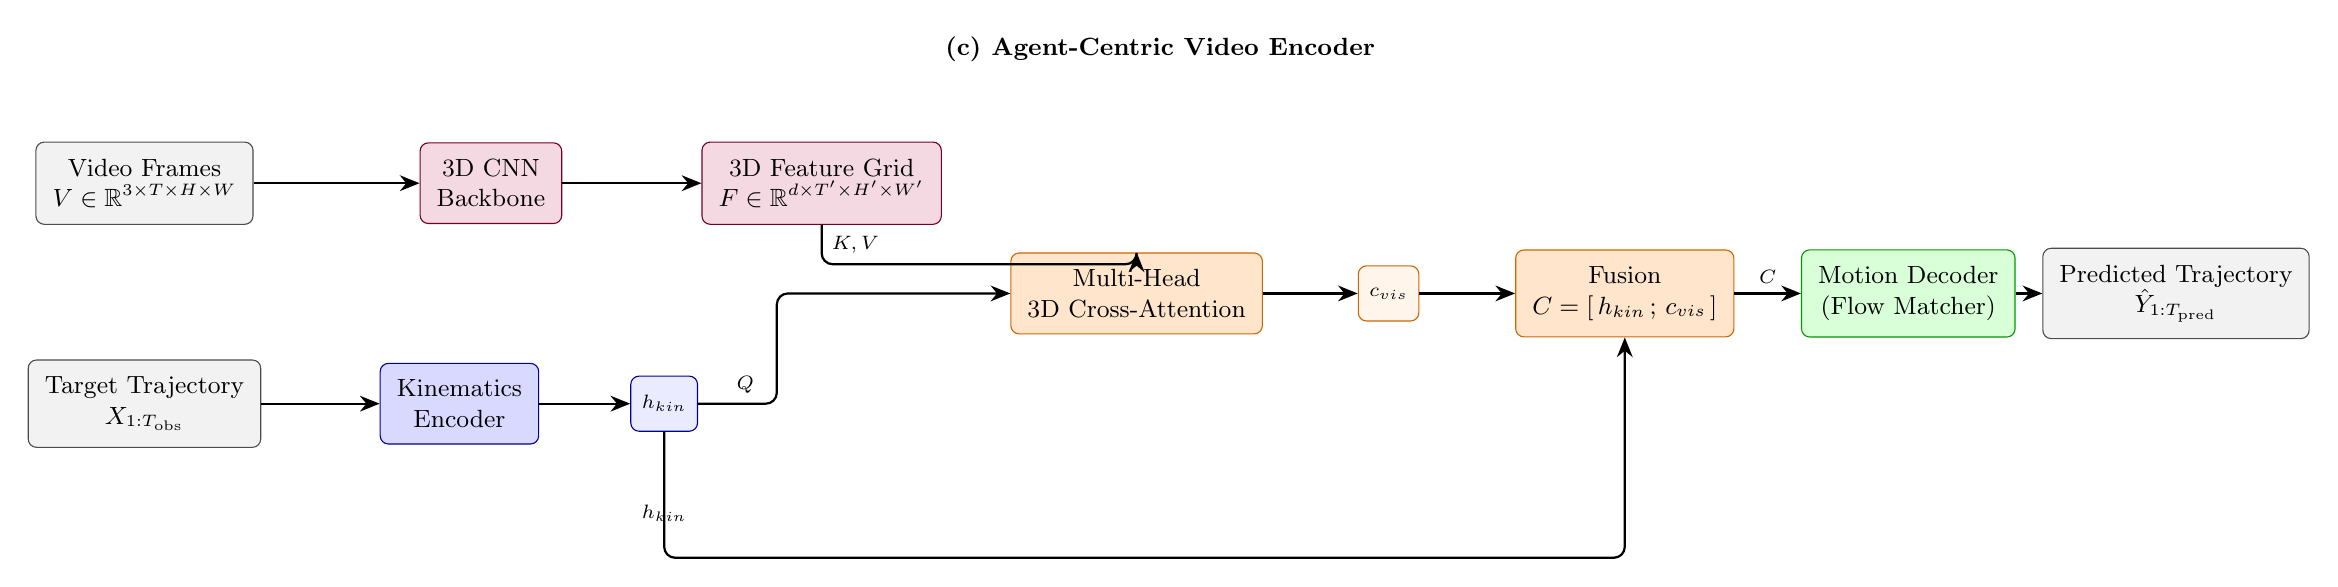
\begin{tikzpicture}
  % ---- target / kinematics stream (bottom row): query ----
  \node[io]  (x)    at (0.0,0.0)  {Target Trajectory\\$X_{1:T_{\mathrm{obs}}}$};
  \node[kin] (kenc) at (4.0,0.0)  {Kinematics\\Encoder};
  \node[vec] (h)    at (6.6,0.0)  {$h_{kin}$};

  % ---- visual stream (top row): keys / values ----
  \node[io]  (v)    at (0.0,2.8)  {Video Frames\\$V\in\mathbb{R}^{3\times T\times H\times W}$};
  \node[vid] (bb)   at (4.4,2.8)  {3D CNN\\Backbone};
  \node[vid] (grid) at (8.6,2.8)  {3D Feature Grid\\$F\in\mathbb{R}^{d\times T'\times H'\times W'}$};

  % ---- attention block + context ----
  \node[fuse] (attn) at (12.6,1.4) {Multi-Head\\3D Cross-Attention};
  \node[veco] (cvis) at (15.8,1.4) {$c_{vis}$};

  % ---- fusion + decoder ----
  \node[fuse] (fus) at (18.8,1.4) {Fusion\\$C=[\,h_{kin}\,;\,c_{vis}\,]$};
  \node[dec]  (dec) at (22.4,1.4) {Motion Decoder\\(Flow Matcher)};
  \node[io]   (y)   at (25.8,1.4) {Predicted Trajectory\\$\hat{Y}_{1:T_{\mathrm{pred}}}$};

  % ---- kinematics + visual stream arrows ----
  \draw[arrow] (x)    -- (kenc);
  \draw[arrow] (kenc) -- (h);
  \draw[arrow] (v)    -- (bb);
  \draw[arrow] (bb)   -- (grid);

  % ---- query / key-value routing into attention ----
  \draw[arrow] (h.east) -- ++(1.0,0)
        node[above, font=\scriptsize, pos=0.6] {$Q$} |- (attn.west);
  \draw[arrow] (grid.south) -- ++(0,-0.5)
        node[right, font=\scriptsize, pos=0.5] {$K,V$} -| (attn.north);

  % ---- attention -> context -> fusion -> decoder -> output ----
  \draw[arrow] (attn) -- (cvis);
  \draw[arrow] (cvis) -- (fus);
  \draw[arrow] (h.south) -- ++(0,-1.6)
        node[below, font=\scriptsize, pos=0.5] {$h_{kin}$} -| (fus.south);
  \draw[arrow] (fus) -- (dec) node[midway, above, font=\scriptsize] {$C$};
  \draw[arrow] (dec) -- (y);

  \node[title] at (12.9,4.5) {(c) Agent-Centric Video Encoder};
\end{tikzpicture}
\end{document}
